\PassOptionsToPackage{sols}{handout}
\documentclass[main]{subfiles}
\setcounterrefbeforedot{chapter}{m-ws2-1}
\setcounterrefafterdot{section}{m-ws2-1}
\addtocounter{section}{-1}
\usepackage{solutions}
\begin{document}

\ifSubfilesClassLoaded{%
  \chaptermark{\chaptertwo}
}{}

\section{Circular Motion, Arc Length, and Angles} \label{ws2-1}

% \begin{objectives}

% Learning Objectives:

% \begin{itemize}[topsep=0pt,partopsep=0pt,parsep=8pt,itemsep=0pt]

% \item You should understand the definition of $\tan x$ and its unit circle
%   interpretation as the slope of the line between the origin and $P(x)$. 

% \item You should understand the graph of $\tan x$ and its connection with
%   the graphs of $\sin x$ and $\cos x$.

% \item You should be comfortable using both radians and degrees to describe
%   angles.

% \item You should understand the relationship between angles and arc
%   length (by ``arc length,'' we mean the length of an arc of a circle).

% \item You should be able to use symmetry and the unit circle to reason
%   about trigonometric values of related angles.  (For example, you should
%   be able to determine how $\sin(\pi - x)$ relates to $\sin x$.)

% \end{itemize}
% \end{objectives}

\textbf{Key Idea}: Circular motion can be described using quantities like radius, arc length, period, and speed.

\begin{enumerate}

\item
\begin{problem}
    Circular motion is everywhere, from particles to people to planets. Let's look at an example. A merry-go-round spinning at a constant rate is an example of \emph{uniform circular motion}. From a top-down perspective, riders trace out circular arcs as the merry-go-round spins, shown below. A rider's distance from the center is the \textbf{radius} $r$ of the circular arc. The length of the arc is called the \textbf{arc length} $s$.
\end{problem}

\begin{minipage}[t]{1.8in}\vspace{0pt}

\includegraphics[width=1.7in]{tikz/2-1/2-1-merry-go-round.pdf}
\end{minipage}
\hfill
\begin{minipage}[t]{4.3in}\vspace{0pt}
\begin{enumerate}
    \item 
    \begin{problem}
    Find the arc length traversed in one full revolution by a rider
    \end{problem}
    \begin{enumerate}
        \item 
        \begin{problem}1\,m from the center\end{problem}\pspace{36pt}
        
        \begin{solution}
            The circumference of a circle with radius 1 m is \fbox{$2\pi$ m.}
        \end{solution}
        
        \item 
        \begin{problem}2\,m from the center\end{problem}
        
                \begin{solution}
            The circumference of a circle with radius 2 m is \fbox{$4\pi$ m.}
        \end{solution}
    \end{enumerate}
\end{enumerate}
\end{minipage}

\begin{enumerate}[start=2]
    \item 
    Find the arc length traversed in half of a revolution by a rider
    \begin{tasks}[before-skip=0pt,label=\roman*.](2)
    \task
    \begin{problem}
        1\,m from the center 
    \end{problem}

    \begin{solution}
        Half of $2\pi$ m is \fbox{$\pi$ m.}
    \end{solution}
    
    \task
    \begin{problem}
        2\,m from the center
    \end{problem}

    \begin{solution}
        Half of $4\pi$ m is \fbox{$2\pi$ m.}
    \end{solution}
    \end{tasks}
    \pspace{\stretch{0.5}}
    


\item 
\begin{problem}
The time needed for one full revolution is called the \textbf{period} $T$.  If the merry-go-round completes exactly 6 revolutions every minute, determine the period of a rider
\end{problem}
    \begin{tasks}[before-skip=0pt,label=\roman*.](2)
    \task
    \begin{problem}
        1\,m from the center 
    \end{problem}

    \begin{solution}
        \fbox{10 seconds}
    \end{solution}
    
    \task
    \begin{problem}
        2\,m from the center
    \end{problem}

    \begin{solution}
        \fbox{10 seconds}
    \end{solution}
    \end{tasks}
    \pspace{\stretch{0.5}}

\item 
\begin{problem}
Since the merry-go-round is spinning at constant rate, we can find a rider's \textbf{speed} $v$ by dividing a distance they travel by the time it takes to cover that distance. Find the speed of a rider
\end{problem}
    \begin{tasks}[before-skip=0pt,label=\roman*.](2)
    \task
    \begin{problem}
        1\,m from the center 
    \end{problem}

    \begin{solution}
        $2\pi$ m divided by 10 s gives \fbox{$\frac{\pi}{5}$ m/s.}
    \end{solution}
    
    \task
    \begin{problem}
        2\,m from the center
    \end{problem}

    \begin{solution}
        $4\pi$ m divided by 10 s gives \fbox{$\frac{2\pi}{5}$ m/s.}
    \end{solution}
    \end{tasks}
    \pspace{\stretch{0.5}}

\item
\begin{problem}
If two people are riding the same merry-go-round at different distances from the center, how are their speeds related, if at all?
\end{problem}
\pspace{\stretch{0.5}}

\begin{solution}
    Two people riding the same merry-go-round will have the same period $T$. However, they will travel different distances in one revolution if their radii are different. For example, as we can see from the previous parts, a person riding 2 m from the center travels twice as far in one revolution as someone riding 1 m from the center, so their speed is twice as large. A rider's speed is proportional to their distance from the center.
\end{solution}

\end{enumerate}
\end{enumerate}

% \begin{framed}
%     \textbf{Circular Motion Key Terms}
%     \begin{itemize}
%         \item radius $r$ is the distance between an object and the center of its circular path.
%         \item arc length $s$ is the distance traveled by the object as it traces out a circular arc.
%         \item period $T$ is the time needed for an object to complete a full revolution.
%         \item speed $v$ is the rate of change of the distance traveled by the object.
%     \end{itemize}
%     When an object travels in a circle at a constant speed, this is called uniform circular motion.
% \end{framed}

\pspace{\newpage}

\textbf{Key Idea}: An angle measures an amount of rotation. It does not depend on distance from the center.

\begin{enumerate}[resume]
    \item 
    \begin{problem}
    Two riders on the same merry-go-round might travel different distances in the same amount of time, since arc length depends on radius. However, they will experience the same ``amount of rotation.'' What were the two different amounts of rotation described in the last problem? What units can we use to describe amount of rotation?
    \end{problem}
    \pspace{\vfill}

    \begin{solution}
        In the previous problem, we found the distance traveled in one revolution and in half of a revolution. These were measured in units of revolutions. However, we can also talk about rotations using units of degrees. One revolution is \ang{360}, and half a revolution ia \ang{180}.
    \end{solution}

    \item 
    We measure amount of rotation by measuring the \textbf{angle} $\theta$ formed at the center by the \emph{initial ray} through a point's initial position and the \emph{terminal ray} through the point's final position.

\begin{minipage}[t]{4.3in}\vspace{0pt}
\begin{enumerate}[nosep]
    \item 
    \begin{problem}
    Draw and label the initial and terminal rays for the rotation shown.
    \end{problem}
    
    \item
    \begin{problem}
    Rotating by the amount shown six times would return all the points to their initial positions. What is the measure of the rotation in
    \end{problem}
    \begin{enumerate}
        \item 
        \begin{problem}
            revolutions?
        \end{problem}
        \pspace{24pt}

        \begin{solution}
            $\frac{1}{6}$ of a revolution
        \end{solution}

        \item 
        \begin{problem}
            degrees?
        \end{problem}

        \begin{solution}
            60 degrees
        \end{solution}
    \end{enumerate}

\end{enumerate}
\end{minipage}
\hfill
    \begin{minipage}[t]{1.8in}\vspace{0pt}
\probonly{
\includegraphics[width=1.7in]{tikz/2-1/2-1-angle-rays.pdf}}
\solonly{
\includegraphics[width=1.7in]{tikz/2-1/2-1-angle-rays-sols.pdf}}
\end{minipage}

\item
\begin{problem}
    Draw the initial and terminal rays for each rotation. Which two angles have the same measure?
\end{problem}
\end{enumerate}
\vspace{-8pt}
    \probonly{
\includegraphics[width=\textwidth]{tikz/2-1/2-1-angle-size.pdf}}
    \solonly{
\includegraphics[width=\textwidth]{tikz/2-1/2-1-angle-size-sols.pdf}}
    \pspace{\stretch{0.2}}

    \begin{solution}
        Angles (a) and (b) have the same measure, both represent a counterclockwise rotation by a quarter-turn. Angle (c) is greater than a quarter-turn, and angle (d) is a clockwise quarter-turn.
    \end{solution}
\begin{enumerate}[resume]
\item
\begin{enumerate}
    \item 
    \begin{problem}
        An angle is in \emph{standard position} when its center is at the origin and its initial ray points in the positive $x$-direction. Which angles in the previous problem were not in standard position?
    \end{problem}
    \pspace{\vfill}

    \begin{solution}
        Angles (a) and (b) were not in standard position. Angles (c) and (d) were in standard position.
    \end{solution}

    \item 
    \begin{problem}
        By convention, we measure counterclockwise rotations with positive angles and clockwise rotations with negative angles. Which of the angles in the previous problem were negative?
    \end{problem}
    \pspace{\vfill}

    \begin{solution}
        Angle (d) is negative. All of the others are positive.
    \end{solution}
\end{enumerate}
\end{enumerate}

\pspace{\newpage}

\textbf{Key Idea}: Radians are a useful unit for measuring angles because of their close connection to arc length.

\begin{enumerate}[resume]
\item
The \textbf{radian} is an angle unit with the property that one full turn or \ang{360} is $2\pi$\,rad. Let's see why this is useful. In each part, determine the measure of the angle \emph{subtended} at the center of the described arc in units of turns, degrees, and radians. Draw the angle in standard position.
\end{enumerate}

\begin{tasks}[before-skip=0pt, label=\roman*., label-width=12pt, after-item-skip=48pt](2)
\task
\begin{problem}
    Radius 1\,cm and arc length $\pi$\,cm.
\end{problem}

\begin{minipage}[t]{1.3in}\vspace{0pt}
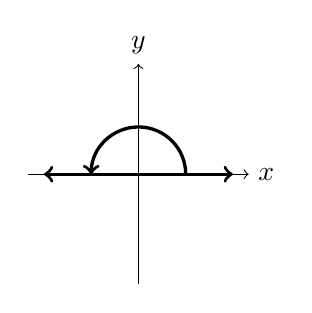
\begin{tikzpicture}[scale=0.4]
    \draw[->] (-3.5,0) -- (3.5,0) node[right] {$x$};
    \draw[->] (0,-3.5) -- (0,3.5) node[above] {$y$};
    \solonly{
    \draw[very thick,->] (1.5,0) arc[start angle=0, end angle=180, radius=1.5];
    \draw[very thick, ->] (0,0) -- (0:3);
    \draw[very thick, ->] (0,0) -- (180:3);
    }
\end{tikzpicture}
\end{minipage}
\hfill
\begin{minipage}[t]{1.5in}\vspace{6pt}
\begin{itemize}[itemsep=16pt]
    \item \cfitb{0.5in}{$\frac{1}{2}$} turns
    \item \cfitb{0.5in}{$180$} degrees
    \item \cfitb{0.5in}{$\pi$} radians
\end{itemize}
\end{minipage}

\task
\begin{problem}
    Radius 7\,in and arc length $7\pi$\,in.
\end{problem}

\begin{minipage}[t]{1.3in}\vspace{0pt}
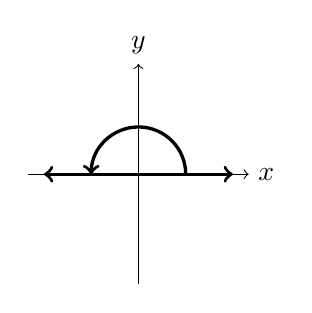
\begin{tikzpicture}[scale=0.4]
    \draw[->] (-3.5,0) -- (3.5,0) node[right] {$x$};
    \draw[->] (0,-3.5) -- (0,3.5) node[above] {$y$};
    \draw[very thick,->] (1.5,0) arc[start angle=0, end angle=180, radius=1.5];
    \draw[very thick, ->] (0,0) -- (0:3);
    \draw[very thick, ->] (0,0) -- (180:3);
\end{tikzpicture}
\end{minipage}
\hfill
\begin{minipage}[t]{1.5in}\vspace{6pt}
\begin{itemize}[itemsep=16pt]
    \item \cfitb{0.5in}{$\frac{1}{2}$} turns
    \item \cfitb{0.5in}{$180$} degrees
    \item \cfitb{0.5in}{$\pi$} radians
\end{itemize}
\end{minipage}


\task
\begin{problem}
    Radius 1\,km and arc length $\frac{\pi}{2}$\,km. 
\end{problem}

\begin{minipage}[t]{1.3in}\vspace{0pt}
\begin{tikzpicture}[scale=0.4]
    \draw[->] (-3.5,0) -- (3.5,0) node[right] {$x$};
    \draw[->] (0,-3.5) -- (0,3.5) node[above] {$y$};
    \draw[very thick,->] (1.5,0) arc[start angle=0, end angle=90, radius=1.5];
    \draw[very thick, ->] (0,0) -- (0:3);
    \draw[very thick, ->] (0,0) -- (90:3);
\end{tikzpicture}
\end{minipage}
\hfill
\begin{minipage}[t]{1.5in}\vspace{6pt}
\begin{itemize}[itemsep=16pt]
    \item \cfitb{0.5in}{$\frac{1}{4}$} turns
    \item \cfitb{0.5in}{$90$} degrees
    \item \cfitb{0.5in}{$\frac{\pi}{2}$} radians
\end{itemize}
\end{minipage}

\task
\begin{problem}
    Radius 3\,mi and arc length $\frac{3\pi}{2}$\,mi.
\end{problem}

\begin{minipage}[t]{1.3in}\vspace{0pt}
\begin{tikzpicture}[scale=0.4]
    \draw[->] (-3.5,0) -- (3.5,0) node[right] {$x$};
    \draw[->] (0,-3.5) -- (0,3.5) node[above] {$y$};
    \draw[very thick,->] (1.5,0) arc[start angle=0, end angle=90, radius=1.5];
    \draw[very thick, ->] (0,0) -- (0:3);
    \draw[very thick, ->] (0,0) -- (90:3);
\end{tikzpicture}
\end{minipage}
\hfill
\begin{minipage}[t]{1.5in}\vspace{6pt}
\begin{itemize}[itemsep=16pt]
    \item \cfitb{0.5in}{$\frac{1}{4}$} turns
    \item \cfitb{0.5in}{$90$} degrees
    \item \cfitb{0.5in}{$\frac{\pi}{2}$} radians
\end{itemize}
\end{minipage}

\task
\begin{problem}
    Radius 1\,m and arc length 1\,m.
\end{problem}

\begin{minipage}[t]{1.3in}\vspace{0pt}
\begin{tikzpicture}[scale=0.4]
    \draw[->] (-3.5,0) -- (3.5,0) node[right] {$x$};
    \draw[->] (0,-3.5) -- (0,3.5) node[above] {$y$};
    \draw[very thick,->] (1.5,0) arc[start angle=0, end angle=57.3, radius=1.5];
    \draw[very thick, ->] (0,0) -- (0:3);
    \draw[very thick, ->] (0,0) -- (57.3:3);
\end{tikzpicture}
\end{minipage}
\hfill
\begin{minipage}[t]{1.5in}\vspace{6pt}
\begin{itemize}[itemsep=16pt]
    \item \cfitb{0.5in}{$\frac{1}{2\pi}$} turns
    \item \cfitb{0.5in}{$\frac{180}{\pi}$} degrees
    \item \cfitb{0.5in}{$1$} radians
\end{itemize}
\end{minipage}

\task
\begin{problem}
    Radius 5\,yd and arc length 5\,yd.
\end{problem}

\begin{minipage}[t]{1.3in}\vspace{0pt}
\begin{tikzpicture}[scale=0.4]
    \draw[->] (-3.5,0) -- (3.5,0) node[right] {$x$};
    \draw[->] (0,-3.5) -- (0,3.5) node[above] {$y$};
    \draw[very thick,->] (1.5,0) arc[start angle=0, end angle=57.3, radius=1.5];
    \draw[very thick, ->] (0,0) -- (0:3);
    \draw[very thick, ->] (0,0) -- (57.3:3);
\end{tikzpicture}
\end{minipage}
\hfill
\begin{minipage}[t]{1.5in}\vspace{6pt}
\begin{itemize}[itemsep=16pt]
    \item \cfitb{0.5in}{$\frac{1}{2\pi}$} turns
    \item \cfitb{0.5in}{$\frac{180}{\pi}$} degrees
    \item \cfitb{0.5in}{$1$} radians
\end{itemize}
\end{minipage}

\end{tasks}

\begin{enumerate}[resume]
\item 
\begin{problem}
Given an arc of length $s$ and radius $r$, how can we calculate the subtended central angle $\theta$ in radians?
\end{problem}
\pspace{\vfill}

\begin{solution}
    Based on the pattern from our work above, the relationship between an angle $\theta$ measured in radians, the radius of a circle $r$, and the arc length $s$ is \[\theta = \frac{s}{r}\]
    Meaning that 1 radian is the subtended angle when an circular arc has the same length as the radius of the circle. We can prove this by setting up a proportion. The ratio of the arc length to the circumference should be the same as the ratio between the subtended angle and $2\pi$ radians (a full turn.)
    \begin{align*}
        \frac{\theta}{2\pi} &= \frac{s}{2\pi r} \\[4pt]
        \theta &= \frac{s}{r}
    \end{align*}
\end{solution}

The relationship that radians provide between lengths and angles is extremely important, so radians are often considered the ``default'' unit for angles. From now on, if you don't see a unit attached to an angle measure, you should assume it is in radians.

\end{enumerate}

\pspace{\newpage}

\textbf{Key Idea}: Reference angles help us locate and draw angles in standard position.

\begin{enumerate}[resume]

\item 
\begin{problem}
Consider the angle $\frac{5\pi}{6}$. How can we figure out how to draw this angle in standard position? Is there a familiar angle nearby we can use as a landmark? What \emph{quadrant} does $\frac{5\pi}{6}$ land in?
\end{problem}
\pspace{\vfill}

\begin{solution}
    $\frac{5\pi}{6}$ is close to but a little less than $\frac{6\pi}{6}$, or $\pi$. This means that $\frac{5\pi}{6}$ will land in quadrant II, like this.
    \begin{center}
\begin{tikzpicture}
    \begin{axis}[
        axis equal image,
        xmin=-5, xmax=5, ymin=-5, ymax=5,
        xlabel={$x$},
        ylabel={$y$},
        xtick=\empty, ytick=\empty,
        width=2.5in
      ]
      % Draw the angle
      \draw[thick,->] (0,0) -- (\rtheta{5}{0});
      \draw[thick,->] (0,0) -- (\rtheta{5}{150});

      % Draw angle arc
      \addplot[domain=0:150,-stealth, very thick] ({cos(x)},{sin(x)});

      % Label the angle
      \node at (\rtheta{1.5}{150/2}) {$\theta$};

      % Label the reference angle
      \node at (\rtheta{2}{170}) {\footnotesize$\pi/6$};

    \end{axis}
\end{tikzpicture}
\end{center}
\end{solution}

\item   \label{2-1-ref-angles}

% \note{You may want to point out that, although $\frac{5 \pi}{2}$ and
%     $\frac{\pi}{2}$ are coterminal, they are not the same.
%     This is important when we solve trig equations; for example, if we're
%     solving $\sin x = 1$ on $[0, \pi]$, then $\frac{\pi}{2}$ is a solution
%     and $\frac{5 \pi}{2}$ is not.}

Given an angle $\theta$ in standard position, its \textbf{reference angle} is the acute angle formed by the terminal ray of $\theta$ and the $x$-axis. In other words, the reference angle measures how far away the angle is from a multiple of $\pi$ or \ang{180}.
For each of the following angles, sketch the angle in standard position by using a reference angle to help you. Convert the angle from radians to degrees, or vice versa.

  {
    \newcommand{\drawcircle}{
      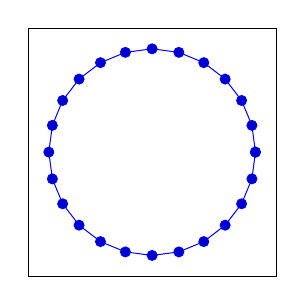
\begin{tikzpicture}[scale=0.9]
        \begin{axis}[width=2in, height=2in, axis equal=true,
        xtick=\empty, ytick=\empty]
          \addplot+[domain=0:360] ({cos(x)}, {sin(x)});
        \end{axis}
      \end{tikzpicture}
    }

    \begin{tabular}{cccc}
      $\displaystyle \frac{2\pi}{3} = \fitb{1cm}{120}^\circ$ &
      $\fitb{1cm}{\frac{7\pi}{6}} = \displaystyle 210^\circ$ & 
      $\displaystyle \frac{7\pi}{4} = \fitb{1cm}{450}^\circ$ &
      $\fitb{1cm}{\frac{13\pi}{6}} = \displaystyle 390^\circ$ \\
      \probonly{\drawcircle}
      \solonly{
        \begin{tikzangle}[angle=2*pi/3]
        \end{tikzangle}        
      }
      &
      \probonly{\drawcircle}
      \solonly{
        \begin{tikzangle}[angle=7*pi/6]

        \end{tikzangle}
      } &
      \probonly{\drawcircle}
      \solonly{
        \begin{tikzangle}[angle=7*pi/4]

        \end{tikzangle}        
      } &
      \probonly{\drawcircle}
      \solonly{
        \begin{tikzangle}[angle=13*pi/6]

        \end{tikzangle}
      }
    \end{tabular}
  }
\pspace{\stretch{0.25}}

\begin{solution}
    Since half a turn is \ang{180} and $\pi$ radians, we can convert between degrees and radians by multiplying by an appropriate conversion factor, like so:
    \begin{itemize}
        \item $\frac{2\pi}{3}\text{ rad} \times \frac{\ang{180}}{\pi\text{ rad}} = \ang{120}$
        \item $\ang{210} \times \frac{\pi\text{ rad}}{\ang{180}} = \frac{7\pi}{6}\text{ rad}$
    \end{itemize}
    We can use reference angles to help us sketch the angles.
    \begin{itemize}
    \item Since $\frac{2\pi}{3}$ is $\frac{\pi}{3}$ less than $\pi$, we know the angle lands in quadrant II.
    \item Since \ang{210} is \ang{30} more than \ang{180}, we know the angle lands in quadrant III.
    \end{itemize}
\end{solution}

\item
\begin{problem}
    Two angles might have the exact same initial ray and terminal ray but not represent the same amount of rotation. These are called \textbf{coterminal angles.} Come up with some examples of coterminal angles.
\end{problem}
\pspace{\vfill}

\begin{solution}
    Any angle $\theta$ and $\theta + 2\pi$ are coterminal. For example, $\frac{\pi}{4}$ and $\frac{9\pi}{4}$. We can continue adding and subtracting multiples of $2\pi$. So $\frac{17\pi}{4}$ and $-\frac{7\pi}{4}$ are also coterminal with $\frac{\pi}{4}$.
\end{solution}

\item   

Follow the same directions as in \ref{2-1-ref-angles}. What do you notice about an angle and its opposite angle?

  {
    \newcommand{\drawcircle}{
      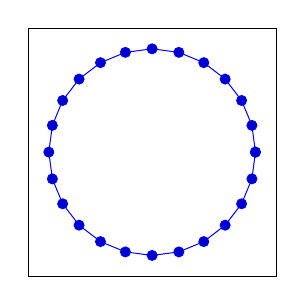
\begin{tikzpicture}[scale=0.9]
        \begin{axis}[width=2in, height=2in, axis equal=true,
        xtick=\empty, ytick=\empty]
          \addplot+[domain=0:360] ({cos(x)}, {sin(x)});
        \end{axis}
      \end{tikzpicture}
    }

    \begin{tabular}{cccc}
      $\displaystyle -\frac{2\pi}{3} = \fitb{1cm}{-120}^\circ$ &
      $\fitb{1cm}{-\frac{7\pi}{6}} = \displaystyle -210^\circ$ & 
      $\displaystyle -\frac{7\pi}{4} = \fitb{1cm}{-450}^\circ$ &
      $\fitb{1cm}{-\frac{13\pi}{6}} = \displaystyle -390^\circ$ \\
      \probonly{\drawcircle}
      \solonly{
        \begin{tikzangle}[angle=-2*pi/3]
        \end{tikzangle}        
      }
      &
      \probonly{\drawcircle}
      \solonly{
        \begin{tikzangle}[angle=-7*pi/6]

        \end{tikzangle}
      } &
      \probonly{\drawcircle}
      \solonly{
        \begin{tikzangle}[angle=-7*pi/4]

        \end{tikzangle}        
      } &
      \probonly{\drawcircle}
      \solonly{
        \begin{tikzangle}[angle=-13*pi/6]

        \end{tikzangle}
      }
    \end{tabular}
  }
\pspace{\stretch{0.25}}

\begin{solution}
    An angle $\theta$ and its opposite angle $-\theta$ are reflections of each other over the $x$-axis.
\end{solution}
  
\end{enumerate}

\newpage

\begin{enumerate}[resume]

\item 
\begin{problem}
Let $\theta$ be an acute angle. Draw it in standard position. You can pick how large $\theta$ should be, but try to make it look different from $\frac{\pi}{4}$. Then draw the angles $\pi+\theta$, $\pi-\theta$, $2\pi-\theta$, and $-\theta$ in standard position.
\end{problem}
\pspace{\vfill}

\begin{solution}
\begin{center}
    \begin{tikzpicture}
    \begin{groupplot}[
        group style={
            group size=3 by 2,
            xlabels at=edge bottom,
            ylabels at=edge left,
            horizontal sep=2cm,
        },
        width=5cm, height=5cm,
        axis equal image,
        xmin=-1, xmax=1, ymin=-1, ymax=1,
        xtick=\empty, ytick=\empty,
        axis lines=middle,
        domain=0:360,
        clip=false
    ]

    % First plot \theta
    \nextgroupplot
        \addplot[domain=0:30,thick,->] ({0.3*cos(x)},{0.3*sin(x)});
        \draw[red,->,thick] (0,0) -- ({cos(30)},{sin(30)});
        \node at (0.7,0.2) {$\theta$};

    % Second plot \pi - \theta
    \nextgroupplot
        \addplot[domain=0:150,thick,->] ({0.3*cos(x)},{0.3*sin(x)});
        \draw[red,->,thick] (0,0) -- ({-cos(30)},{sin(30)});
        \node at (0.4,0.4) {$\pi - \theta$};

    % Third plot \pi + \theta
    \nextgroupplot
        \addplot[domain=0:210,thick,->] ({0.3*cos(x)},{0.3*sin(x)});
        \draw[red,->,thick] (0,0) -- ({-cos(30)},{-sin(30)});
        \node at (-0.4,0.4) {$\pi + \theta$};

    % Fourth plot 2\pi - \theta
    \nextgroupplot
        \addplot[domain=0:330,thick,->] ({0.3*cos(x)},{0.3*sin(x)});
        \draw[red,->,thick] (0,0) -- ({cos(330)},{sin(330)});
        \node at (-0.4,-0.4) {$2\pi - \theta$};

    % Fifth plot -\theta
    \nextgroupplot
        \addplot[domain=-30:0,thick,<-] ({0.3*cos(x)},{0.3*sin(x)});
        \draw[red,->,thick] (0,0) -- ({cos(-30)},{sin(-30)});
        \node at (0.7,-0.2) {$-\theta$};

    \end{groupplot}
\end{tikzpicture}
\end{center}
\end{solution}
\item The angles below will appear frequently, so you should get familiar with them. Label each point with the corresponding angle measure in radians on the left and degrees on the right. Use positive angles less than one full turn. You may want to practice this exercise until you can locate these angles quickly. 

\end{enumerate}
\begin{center}
\begin{tabular}{cc}
    \begin{tikzpicture}
      
  \begin{axis}[
  xmin=-1.1, xmax=1.1,
  ymin=-1.1, ymax=1.1,
  xlabel=\large$x$, ylabel=\large$y$,
  xtick=\empty, ytick=\empty,
  axis equal = true
  ]
  \coordinate (O) at (0,0);
  \coordinate (X) at (1,0);
  \coordinate (Y) at (0,1);
  \addplot[domain=0:360, data cs=polar] (x,1);
  \end{axis}
  \begin{scope}[x={($(X)-(O)$)}, y={($(Y)-(O)$)}, shift={(O)}]
    \foreach \A in {0,90,180,270} {
      \filldraw[radius=2pt] (\rtheta{1}{\A}) circle;
    }
    \foreach \A in {45, 135, 225, 315} {
      \filldraw[radius=2pt] (\rtheta{1}{\A}) circle;
    }
    \solonly{
    \node[above right] at (0:1) {$0$};
    \node[above right] at (45:1) {$\pi/4$};
    \node[above right] at (90:1) {$\pi/2$};
    \node[above left] at (135:1) {$3\pi/4$};
    \node[below left] at (180:1) {$\pi$};
    \node[below left] at (225:1) {$5\pi/4$};
    \node[below right] at (270:1) {$3\pi/2$};
    \node[below right] at (315:1) {$7\pi/4$};
    }
  \end{scope}
  
\end{tikzpicture} &
\begin{tikzpicture}
      
  \begin{axis}[
  xmin=-1.1, xmax=1.1,
  ymin=-1.1, ymax=1.1,
  xlabel=\large$x$, ylabel=\large$y$,
  xtick=\empty, ytick=\empty,
  axis equal = true
  ]
  \coordinate (O) at (0,0);
  \coordinate (X) at (1,0);
  \coordinate (Y) at (0,1);
  \addplot[domain=0:360, data cs=polar] (x,1);
  \end{axis}
  \begin{scope}[x={($(X)-(O)$)}, y={($(Y)-(O)$)}, shift={(O)}]
    \foreach \A in {0,90,180,270} {
      \filldraw[radius=2pt] (\rtheta{1}{\A}) circle;
    }
    \foreach \A in {45, 135, 225, 315} {
      \filldraw[radius=2pt] (\rtheta{1}{\A}) circle;
    }
    \solonly{
    \node[above right] at (0:1) {$0$};
    \node[above right] at (45:1) {$\ang{45}$};
    \node[above right] at (90:1) {$\ang{90}$};
    \node[above left] at (135:1) {$\ang{135}$};
    \node[below left] at (180:1) {$\ang{180}$};
    \node[below left] at (225:1) {$\ang{225}$};
    \node[below right] at (270:1) {$\ang{270}$};
    \node[below right] at (315:1) {$\ang{315}$};
    }
  \end{scope}
  
\end{tikzpicture}
\end{tabular}

\begin{tabular}{cc}
    \begin{tikzpicture}
      
  \begin{axis}[
  xmin=-1.1, xmax=1.1,
  ymin=-1.1, ymax=1.1,
  xlabel=\large$x$, ylabel=\large$y$,
  xtick=\empty, ytick=\empty,
  axis equal = true
  ]
  \coordinate (O) at (0,0);
  \coordinate (X) at (1,0);
  \coordinate (Y) at (0,1);
  \addplot[domain=0:360, data cs=polar] (x,1);
  \end{axis}
  \begin{scope}[x={($(X)-(O)$)}, y={($(Y)-(O)$)}, shift={(O)}]
    \foreach \A in {0,90,180,270} {
      \filldraw[radius=2pt] (\rtheta{1}{\A}) circle;
    }
    \foreach \A in {60, 150, 210, 330} {
      \filldraw[radius=2pt] (\rtheta{1}{\A}) circle;
    }
    \foreach \A in {30, 120, 240, 300} {
      \filldraw[radius=2pt] (\rtheta{1}{\A}) circle;
    }
    \solonly{
    \node[above right] at (0:1) {$0$};
    \node[above right] at (30:1) {$\pi/6$};
    \node[above right] at (60:1) {$\pi/3$};
    \node[above right] at (90:1) {$\pi/2$};
    \node[above left] at (120:1) {$2\pi/3$};
    \node[above left] at (150:1) {$5\pi/6$};
    \node[below left] at (180:1) {$\pi$};
    \node[below left] at (210:1) {$7\pi/6$};
    \node[below left] at (240:1) {$4\pi/3$};
    \node[below right] at (270:1) {$3\pi/2$};
    \node[below right] at (300:1) {$5\pi/3$};
    \node[below right] at (330:1) {$11\pi/6$};
    }
  \end{scope}
  
  \end{tikzpicture} &
      \begin{tikzpicture}
      
  \begin{axis}[
  xmin=-1.1, xmax=1.1,
  ymin=-1.1, ymax=1.1,
  xlabel=\large$x$, ylabel=\large$y$,
  xtick=\empty, ytick=\empty,
  axis equal = true
  ]
  \coordinate (O) at (0,0);
  \coordinate (X) at (1,0);
  \coordinate (Y) at (0,1);
  \addplot[domain=0:360, data cs=polar] (x,1);
  \end{axis}
  \begin{scope}[x={($(X)-(O)$)}, y={($(Y)-(O)$)}, shift={(O)}]
    \foreach \A in {0,90,180,270} {
      \filldraw[radius=2pt] (\rtheta{1}{\A}) circle;
    }
    \foreach \A in {60, 150, 210, 330} {
      \filldraw[radius=2pt] (\rtheta{1}{\A}) circle;
    }
    \foreach \A in {30, 120, 240, 300} {
      \filldraw[radius=2pt] (\rtheta{1}{\A}) circle;
    }
    \solonly{
    \node[above right] at (0:1) {$0$};
    \node[above right] at (30:1) {$\ang{30}$};
    \node[above right] at (60:1) {$\ang{60}$};
    \node[above right] at (90:1) {$\ang{90}$};
    \node[above left] at (120:1) {$\ang{120}$};
    \node[above left] at (150:1) {$\ang{150}$};
    \node[below left] at (180:1) {$\ang{180}$};
    \node[below left] at (210:1) {$\ang{210}$};
    \node[below left] at (240:1) {$\ang{240}$};
    \node[below right] at (270:1) {$\ang{270}$};
    \node[below right] at (300:1) {$\ang{300}$};
    \node[below right] at (330:1) {$\ang{330}$};
    }
  \end{scope}
  
  \end{tikzpicture}
\end{tabular}
\end{center}

\pspace{\newpage}

\begin{enumerate}[resume]
  
  \item
  \begin{problem}
    The picture shows a circular sector (a wedge of a circle, not to scale.)  The radius is 20 feet, and the central angle is $\frac{\pi}{6}$ radians. What is the length of the bolded arc? 

    \begin{tikzpicture}[x=1.5cm, y=1.5cm]
      \draw (0, 0) -- (110: 2);
      \draw (0, 0) -- node[anchor=north east]{20\,ft} (140: 2);
      \draw[very thick] (110:2) arc[radius=2, start angle=110, end
      angle=140];
      \draw (110:8pt) arc[radius=8pt, start angle=110, end angle=140];
      \draw (125:9pt) node[inner sep=0, pin={[pin edge={black,
          <-}]60,inner sep=0pt:$\dfrac{\pi}{6}$}] {};
    \end{tikzpicture}
  \end{problem}

  \begin{solution}
    Using our formula from part (b), the arc length is $r\theta=20\cdot
    \frac{\pi}{6}=\boxed{\frac{10\pi}{3}}$.
    
    Another approach is to think about what proportion of
    a whole circle we have.  A whole circle would subtend an angle of $2
    \pi$, so we have $\frac{\pi/6}{2 \pi} = \frac{1}{12}$ of a whole
    circle.  The circumference of a circle of radius 20 is $2 \pi \cdot 20
    = 40 \pi$, so $\frac{1}{12}$ of this is $\frac{1}{12} \cdot 40 \pi =
    \boxed{ \frac{10 \pi}{3}}$.     
  \end{solution}


\item  A \emph{nautical mile} is the distance along the surface of the Earth
  that subtends an angle at Earth's center measuring 1 minute of arc, which is equal to $\frac{1}{60}$ degrees.
  \begin{enumerate}
  \item
    \begin{problem}[\vfill]
      Draw a picture to illustrate a nautical mile. How many radians is 1 minute of arc?
    \end{problem}

    \begin{solution}
      Here's a sketch (not to scale):
      \begin{center}
        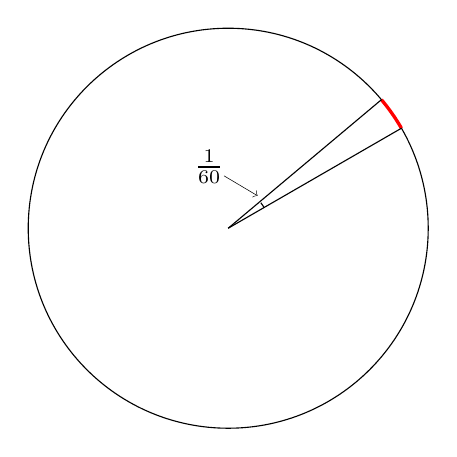
\begin{tikzpicture}[x=1in, y=1in]
          \draw (0, 0) circle (1);
          \draw[red, very thick] (30:1) arc[radius=1, start angle=30, end angle=40];
          \draw (0, 0) -- (30:1);
          \draw (0, 0) -- (40:1);
          \draw (30:15pt) arc[radius=12pt, start angle=30, end angle=40];
          \draw (45:16pt) node[inner sep=0, pin={[pin edge={black,
              <-}]160,inner sep=0pt:$\frac{1}{60}\si{\degree}$}] {};          
        \end{tikzpicture}
      \end{center}
      The circle represents the circumference of the earth, and a nautical
      mile is shown in red.

      Since $\pi$ radians is the same as $180^\circ$, $\frac{1}{60}\si{\degree} = 
      \left( \frac{\pi \text{ radians}}{\ang{180}}
      \right) \frac{1}{60}\si{\degree} = \frac{\pi}{180 \cdot 60} \text{
        radians} = \boxed{\tfrac{\pi}{10800} \text{ radians}}$.
    \end{solution}

  \item
    \begin{problem}[\vfill]
      Earth's radius is about 3960 miles. Use this to approximate
      the length of a nautical mile in \textbf{feet}. (1 mile $=$
      5280 feet.)      
    \end{problem}

    \begin{solution}
      As in {{\#4}}, the key is to think about what
      proportion of an entire circle we have.  Since the angle subtended
      by a nautical mile is $\frac{\pi}{10800}$ and the angle subtended by
      an entire circle is $2 \pi$, a
      nautical mile is $\frac{\pi/10800}{2 \pi}$ of the whole
      circumference of the earth, so
      \begin{align*}
        1 \text{ nautical mile} &= \underbrace{\frac{\pi/10800}{2
            \pi}}_{\text{proportion of circle}} \cdot \underbrace{2 \pi
          \cdot 3960 \text{ miles}}_{\text{circumference of earth}} \\
        &= \frac{3960 \pi}{10800} \text{ miles} \\
        &= \left( \frac{3960 \pi}{10800} \text{ miles} \right)(5280 \text{
          feet/mile}) \\
        &= \boxed{1936 \pi \text{ feet}}
      \end{align*}      
    \end{solution}

  \end{enumerate}

\item 
\begin{problem}
    Geostationary satellites orbit in circles high above the Earth with an orbital period of 24 hours, so they always remain above the same spot on the ground. They travel at a speed of about 3 kilometers per second. Using this information, determine the radius of a geostationary satellite's orbit.
\end{problem}
\pspace{\vfill}

\begin{solution}
    Using the information given, we can determine the circumference of a geostationary satellite's orbit, which we can use to find the radius.

    Since we know that the satellite travels at a speed of 3 km/s and has a period of 24 hours or 86,400 seconds, this means that the satellite travels
    \[\left(\SI{3}{\kilo\meter\per\second}\right)(\SI{86400}{\second}) = \SI{259200}{\kilo\meter}\]
    in one full revolution. This means that the radius of the orbit is
    \[\frac{259200}{2\pi}\,\si{\kilo\meter} \approx \fbox{\SI{41253}{\kilo\meter}.}\]
\end{solution}

\end{enumerate}

\end{document}